\documentclass[main.tex]{subfiles}
\begin{document}
\onlyinsubfile{\mainmatter{}}

\chapter{Background: Ensuring Memory Safety using Capabilities} \label{ch:cheri}
Most security bugs classified as \enquote{serious} in large projects such as the Chromium browser engine \cite{chromium} are memory safety bugs — bugs such as out-of-bounds array or call stack accesses that arise from the use of \enquote{memory-unsafe} programming languages like C, the use of memory safety opt-outs (such as Rust’s \texttt{unsafe}) in \enquote{memory-safe} programming languages, bugs in the compiler, bugs in the standard library implementation of a memory-safe programming language, or bugs in the runtime environment such as the Java VM or an ECMAScript interpreter.

Common approaches to mitigating attacks or restricting the attack vector that such a bug can cause include reintroducing compiler-inserted array bounds checks in memory-unsafe programming languages and enforcing page-level permissions in the virtual memory system of the operating system. However, runtime checks introduce a runtime cost, and virtual memory protection doesn’t protect against a compromised or vulnerable library such as Apache Log4j accessing potentially sensitive data in the process’ address space such as TLS session keys stored in an in-process OpenSSL data structure.

A different approach are \textbf{capabilities}, which are usually unforgeable pointers that carry authority over a precise region of memory and with a precise set of permissions, thereby providing fine-grained memory protection. To ensure that authority cannot be created, capabilities can only be derived from a source with more authority, such as an operating system, a more privileged routine, or another capability. Finally, capability support can be provided at the hardware level, removing the runtime cost associated with software-based bounds \& permission checks.

\shb{Mention that virtual memory offers coarse-grained memory protection, this makes the advantage of (fine-grained mem. prot.) of capabilities hit home}
\shb{You give a general introduction of capabilities (i.e., not CHERI-specific until the next section), but no way of verifying what you mention in the last paragraph to be true. I'd expect a reference to [Levy, Capability-based computer-systems]}
\shb{Maybe: have the last paragraph flow better into the CHERI subsection, i.e., capabilities have been around since 1960, died out, revived in 2014? by CHERI, ... or smth like that (This is a typical intro to capabilities to point out that this is not new, can be implemented in many different ways, ...)}

\section{Capability Hardware Enhanced RISC Instructions}
\textbf{CHERI} (\textbf{Capability Hardware Enhanced RISC Instructions}; see also \cite{intro2cheri}) is a design for a capability machine, extending several existing instruction set architectures (ISAs) such as RISC-V, MIPS, x86-64, and Arm with hardware capability support. One of CHERI’s design goals is to provide a viable transition path for mainstream systems. An ecosystem formed around CHERI, such as capability extensions for C \& C++, capability support in the LLVM compiler toolchain and QEMU emulator, a FreeBSD fork with capability support called CheriBSD, and several large libraries and systems such as PostgreSQL and WebKit being ported to CheriBSD.
\shb{While it's useful to mention the ecosystem, it doesn't convince me from a viable transition path, but of tooling support to start writing cheri-targeted programs. Short summary of the different execution modes (conventional, hybrid, pure-cap) would be appropriate here}

In 64-bit CHERI-RISC-V, the CHERI extension of the 64-bit RISC-V ISA, 64-bit pointers become 128-bit capabilities. As illustrated in \cref{fig:chericoncentrate}, such a capability consists of a 64-bit address, a 27-bit compressed value indicating the capability’s bounds \shb{relative to the address}, a 16-bit permissions mask (specifying permissions such as \emph{permit load}), with the remaining 21 bits reserved for encoding other flags and the capability’s object type (used for a CHERI feature called \enquote{\gls*{sealing}}, cf. infra). A 1-bit validity tag stored out-of-band in tagged memory is set when the 128-bit datum represents a valid capability, and cleared whenever the datum is modified by any instruction not intended to validly modify capabilities (such as \texttt{XOR} or \texttt{ADD}).
\shb{The last sentence is leaving out tagging of registers. (important for the xor/add/... instructions ;)}

CHERI-RISC-V defines several capability-aware instructions that can validly modify capability within specified constraints. For instance, \texttt{CAndPerm} removes permissions from a given capability by performing a bitwise conjunction with a given permissions mask whereas \texttt{CIncOffset} adds an offset to a given capability's address. These limitations are in place to ensure 4 important safety properties of capability machines and CHERI architectures in particular, briefly summarised here below.

\shb{I don't like the "validly modified" term, more common is "guarded manipulation"}

\begin{figure}
	\centering
	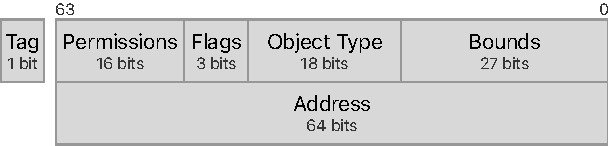
\includegraphics{Images/CHERI Concentrate Layout.pdf}
	\caption{A simplified layout of a 256-bit CHERI capability compressed into 128 bits using the CHERI Concentrate encoding. CHERI-RISC-V defines one flag bit and reserves the other two bits for future use. The validity tag bit is stored out-of-band, usually in tagged memory not directly accessible by user programs.}
	\label{fig:chericoncentrate}
\end{figure}

\paragraph{Permissions} A capability specifies zero or more permissions that the holder of the capability is allowed to do using that capability. \shb{nit: "allowed to do..." -> "allowed to exercise."} For example, the \emph{permit load} resp. \emph{permit store} permissions allow the holder to load resp. store data in the region of memory specified by the capability. Beyond permissions also found in traditional virtual memory systems, capabilities also support CHERI-specific permissions such as \emph{allow local capability store} and \emph{permit seal}. \shb{At this point the reader is unfamiliar with local/sealed caps, you could opt to just use the load-cap, store-cap perms instead} Performing an action not allowed by the capability, such as storing data using a load-only capability, results in a machine trap.\footnote{In some specific cases, such as loading a capability using a capability that only allows loading data but not capabilities, merely results in a capability's tag being cleared, thereby deactivating any authority that it otherwise might unintentionally have conferred.}

\paragraph{Bounds} A capability specifies a contiguous region of memory where the holder of the capability is allowed exercise actions permitted by the capability's permissions. For example, a capability produced by a secure, capability-aware implementation of \texttt{malloc} pointing to a heap-allocated buffer would only permit accesses within that buffer. Performing an action outside of these bounds, i.e., a buffer overflow, results in a machine trap.

\paragraph{Provenance} A capability can only be derived from other capabilities. Authority cannot be forged by modifying its in-memory representation; attempting to do so causes the capability's tag bit to be cleared which invalidates the capability. Tag bits cannot be set in software.

\paragraph{Monotonicity} A capability cannot have more authority than the capability it's derived from: permissions can only be removed and bounds can only be shrunk. At CPU reset, the hardware provides root capabilities to the bootloader or firmware, which can be iteratively restricted in higher levels of abstraction, as illustrated in \cref{fig:derivingauth}.

\begin{figure}
	\centering
	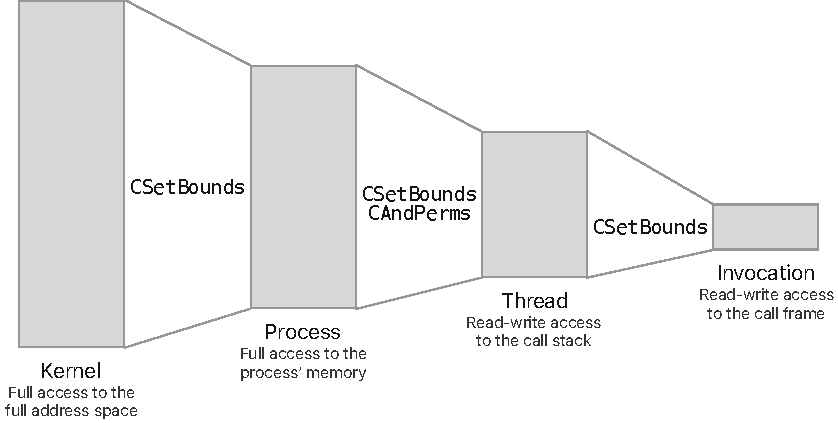
\includegraphics{Images/Deriving Authority.pdf}
	\caption{Provenance and monotonicity in action in protecting process memory, the call stack, and a call frame. The size of the depicted memory regions are not to scale. Similar illustrations can be made about a process' heap and heap-allocated memory.}
	\label{fig:derivingauth}
\end{figure}

\section{Sealed Capabilities}
CHERI provides a capability protection mechanism called \textbf{\gls{sealing}}, whereby the capability holder is restricted from modifying or dereferencing the capability. The inverse operation, i.e., \textbf{\gls{unsealing}}, is only allowed under specific circumstances. \Gls{sealing} comes in two forms: \gls{sealing} using a \gls{sealcap} or \gls{sealing} as a \gls{sentry}. The sealed state of a capability is encoded in its \textbf{object type} field; the object type of an unsealed capability has the special value $-1$.

\paragraph{Sealing using a seal capability} A capability with the \emph{permit seal} permission, i.e., a \textbf{\gls{sealcap}}, can be used to seal another capability. The object type of the sealed capability is set to the \gls{sealcap}'s \enquote{address}.\footnote{Note that this \enquote{address} doesn't necessarily need to refer to a valid location in memory. A capability whose address is only used for sealing and unsealing capabilities should therefore omit the \emph{permit load} and \emph{permit store} family of permissions to avoid letting holders of the seal capability access invalid memory locations.} A capability with the \emph{permit unseal} permission, i.e., an \textbf{\gls{unsealcap}}, can be used to unseal a sealed capability provided that the sealed capability's object type matches the unseal capability's \enquote{address} exactly. A \gls{sealcap} can also act as an \gls{unsealcap} if it has both permissions.
\shb{devils advocate: the address is 64-bits and otype 18-bits, how can we seal with this and how can we unseal (you mention it should *match exactly*)}

As would be expected from normal pointer-like capabilities, the (un)seal capability's address must be within its bounds when (un)sealing; otherwise a machine trap ensues. By carefully controlling access to and bounding capabilities with the \emph{permit seal} and \emph{permit unseal} permissions, sealing can be used for higher-level features such as encapsulation.

Sealing and unsealing can be done using the \texttt{CSeal} respectively \texttt{CUnseal} instructions. CHERI-RISC-V additionally provides a \texttt{CInvoke} instruction that takes a code and data capability pair with matching object type, unseals them, and jumps to the code capability's address. This feature enables secure domain transitions, wherein the caller cannot dereference the code or data capability (which may belong to a closure, for example), but can use them to perform an invocation.

\paragraph{Sealing as a sentry capability} An executable capability can be sealed by itself as a \textbf{\gls{sentry}} using the \texttt{CSealEntry} instruction. CHERI-RISC-V defines a \texttt{CJALR} instruction that jumps to the address of a given target capability, unsealing the capability if it is a \gls{sentry}. Similar to RISC-V's \texttt{JALR} instruction, the instruction also accepts a link register wherein it puts the return address. Unlike \texttt{JALR} however, \texttt{CJALR} also seals the return capability as a \gls{sentry}, ensuring that the callee can only use it to return to the caller. A \gls{sentry}'s object type has the special value $-2$.

\biblio{}
\onlyinsubfile{\glsaddall\printglossaries}
\end{document}
